\documentclass[SoftwareQuality.tex]{subfiles}


\begin{document}

\section{Why do we concern?} 



\subsection*{costs of failures}
\begin{frame}{Relative costs of Software failures} 
How expensive are failures depending on the time they are recovered:
\vfill
\begin{tabular}{l r}
 while developing a feature & { 1}\\ 
  {when developer tests the completed feature}  & \visible<2->3\\
  {while integration testing}   & \visible<3->{10}\\
  {while QA testing}  & \visible<4->{100}\\
  {in production} &   \visible<5->{1000}\\
\end{tabular} 
\end{frame}

\subsection*{problems of manual tests}
\begin{frame}{Why are manual tests flaky?} 
Testing software manually has some serious influences:
\vfill 

\visible<2->{
Software must be ready to run.
}

\vfill 
\visible<3->{ Tester needs knowledge about complete Application. 
\\\hspace{3em}what is desired behavior? 
\\\hspace{3em} what is a failure?
}
\vfill 
\visible<4->{ 
 Testing failure handling my be hard.
}
\vfill 
\visible<5->{ 
 Testing is slow.
}

\vfill 
\visible<6->{ 
Testing only during business hours.
}

\vfill 
\visible<7->{ 
 Testing is boring.
 }
\end{frame}

\subsection*{alternative to manual tests}
\begin{frame}{How to make it better?} 
Computers are good in:
\begin{itemize}
	\item  doing things that have clear input and output
	\item  doing things that have rules to make decisions
	\item  repeating tasks
\end{itemize}
\vfill

\visible<2->{
Tests 
\begin{itemize}
	\item  have  clear input and output
	\item  have rules when passing or failing
	\item  must be repeated regularly
\end{itemize}}
\vfill

\visible<3->{ \Large Automate your tests!}
\end{frame}

\subsection*{What kind of test should we automate?}
\begin{frame}{Test Level} 

\begin{itemize}
	\item Application Test
		\begin{itemize}
			\item rejection check {\color{gray}formaly known as \textit{acceptance test}}.
			\item performance/stress test
		\end{itemize}
	\item Module Test
	\item Unit Test
\end{itemize}

\end{frame}

\begin{frame}{Application Test} 
\begin{itemize}
\item testing the Application as a whole.
\item act as the (end-) user.
\item control via (graphical) user interface.
\item many tests needed to cover all functionality.
\item some functionality is implicitly tested multiple times.
\item any desired change may break multiple test.
\item failing test gives almost no information about the cause of the fail.
\item proves that all modules work together.
%\item somewhat faster that manual tests.
\end{itemize}

\end{frame}


\begin{frame}{Module Test} 
\begin{itemize}
\item testing an isolated Module.
\item control via Module API.
\item many tests needed to cover all functionality of the module.
\item some functionality is implicitly tested multiple times.
\item any desired change of the module may break multiple test.
\item failing test gives almost no information about the cause of the fail.
\item proves that all units work together.
\item somewhat faster that Application Tests.
\end{itemize}

\end{frame}

\begin{frame}{UnitTest} 
\begin{itemize}
\item testing an isolated Unit.
\item testing a single assumption about the Unit.
\item control via Unit API.
\item few tests per unit needed to cover all functionality.
\item \textit{no} functionality is implicitly tested multiple times.
\item failing test gives detailed information about the cause of the fail.
\item very fast.
\end{itemize}

\end{frame}

\begin{frame}{Conclusion} 
Any level of test can be automated, but:
\vfill

\textbf{Applications an Module  Test}
\begin{itemize}
\item run late in the development process
\item need tooling complex API
\item are fragil
\end{itemize}

\textbf{UnitTest}
\begin{itemize}
\item run early in the development process
\item need tooling with simple API
\item are stable
\end{itemize}
%\vfill

With high UnitTest coverage less higher level  tests are needed.

UnitTests check the functionality.

Higher level tests check that all works together smoothly.

\end{frame}

\begin{frame}{Why don't we write automated tests?} 
\pause
\visible<2>{
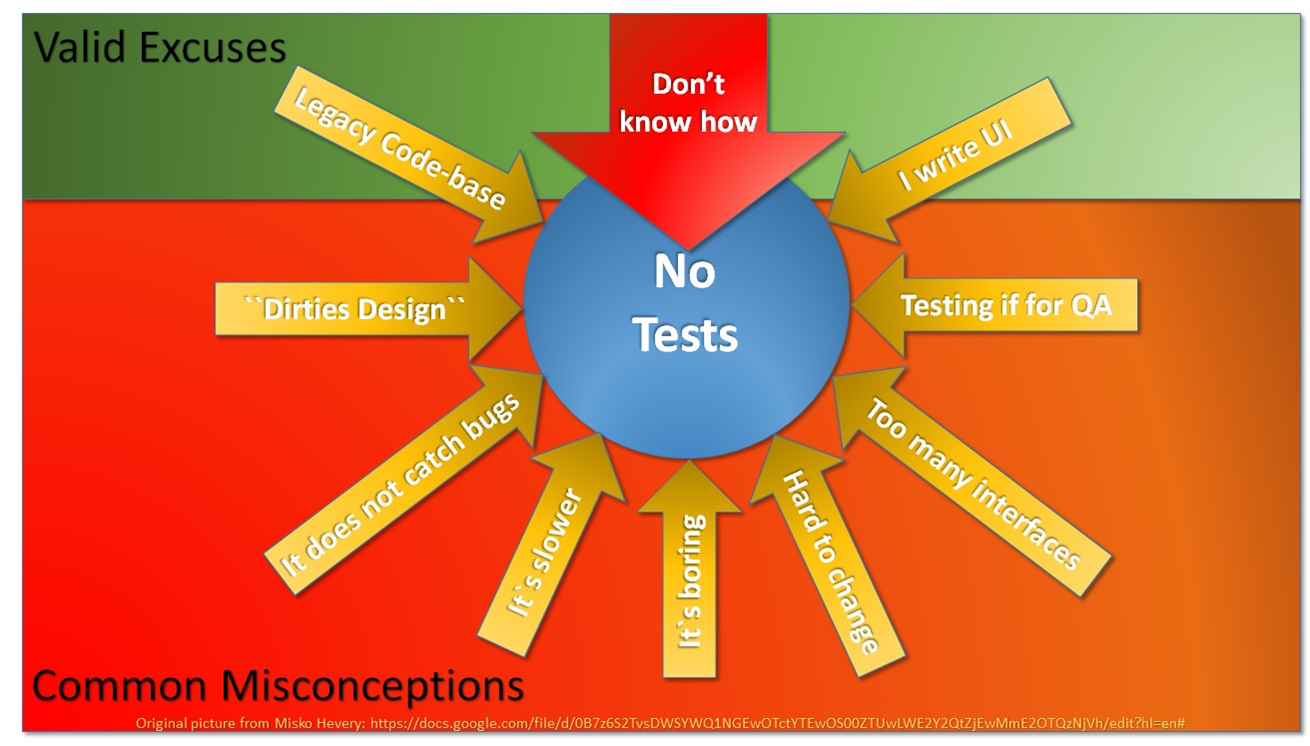
\includegraphics[scale=.5]{excuses}
}
\end{frame}

\begin{frame}{UnitTests as a skill} 

{\Huge
Writing UnitTests is a skill that needs to be trained constantly.}
\vfill
Next chance: 
\\Global Day of Coderetreat Oktober 22nd at HS Fulda\\
\footnotesize\url{http://coderetreat.org/events/global-day-of-coderetreat-2016-fulda-germany}

\end{frame}
\end{document}